\chapter{Entwicklung und Simulation von Anwendungsprogrammen}\label{ch:Entwicklung und Simulation des Frontends}
\section{Entwurf der Smartphone-App}\label{sec:Entwurf der Android-App}

\begin{wrapfigure}{r}{0.5\textwidth}
    \centering
    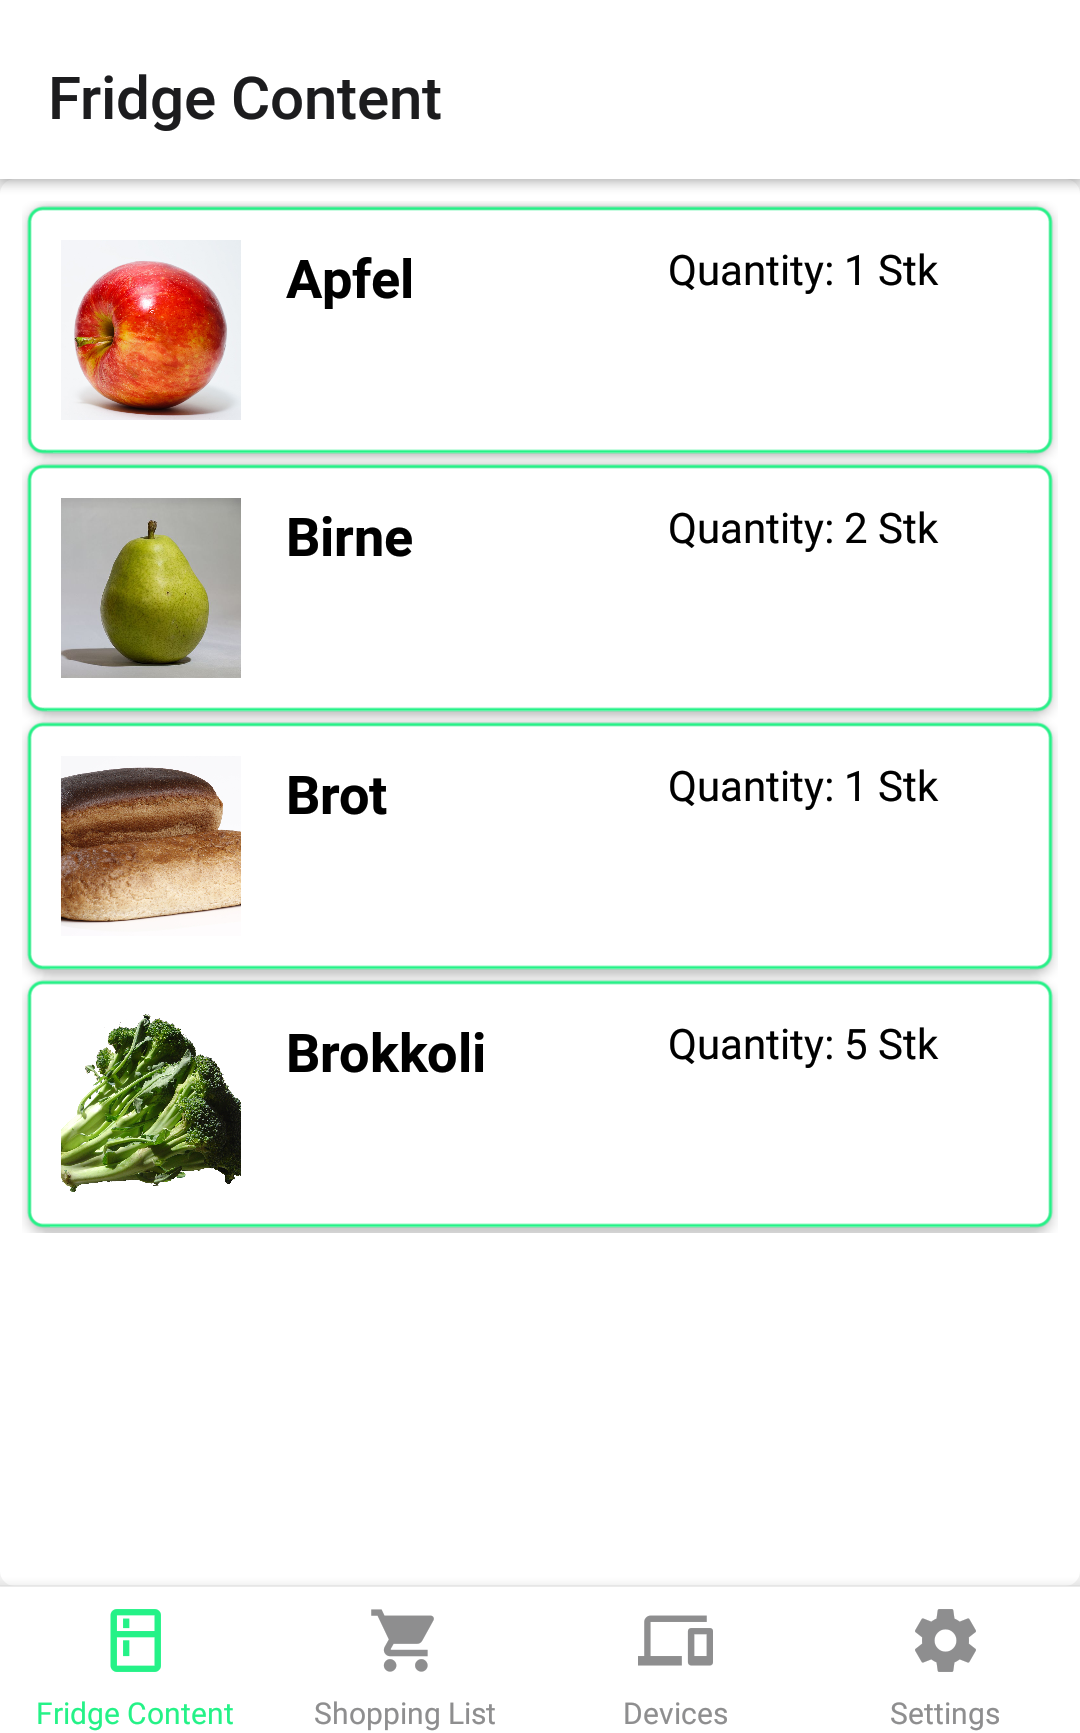
\includegraphics[width=0.4\textwidth]{figures/4.1.png}
    \caption{Layout der Smartphone-App}
    \label{fig:4.1}
\end{wrapfigure}

Im Rahmen dieser Arbeit wird bereits ein erster Prototyp der späteren Smartphone-App entwickelt. Für die Entwicklung wird das React-Native-Framework verwendet, da dieses die Möglichkeit bietet mit einer Codebasis sowohl für Android als auch für iOS zu entwickeln. Die Entwicklung der App erfolgt wie auch im Backend mit der Programmiersprache TypeScript.\\ Da es sich bei der App lediglich um einen Prototyp handelt, wird auf eine vollständige Implementierung aller späteren Funktionen verzichtet. Die primäre Aufgabe der App ist es, die Funktion des Backends zu testen und die Ergebnisse zu präsentieren. In Abbildung~\ref{fig:4.1} das aktuelle Layout der App dargestellt. Es wird nur die dargestellte \textit{Fridge Content}-Ansicht verwendet. Aus dem Backend werden die Daten aller Produkte die sich in den Geräten der Benutzerin bzw. des Benutzers befinden geladen und angezigt.

\section{Simulation von Drittsystemen}\label{sec:Simulation von Drittsystemen}

Alle nicht nicht in der App implementierten Funktionen, die für den Betrieb des Prototypen benötigt werden, werden mit Hilfe eines in Python geschriebenen \glsxtrfull{CLI} simuliert. Mit diesem ist es Möglich sowohl administrative Aufgaben, wie das Anlegen neuer Produktklassen oder Einheiten zu erledigen, als auch Aktionen die durch Benutzer:innen ausgeführt werden zu simulieren. Alle diese Funktionen werden durch die Verwendung der \gls{REST-API} des Backend-Servers ausgeführt. In zukünftigen Versionen können die Schnittstellen durch die Smartphone-App oder durch ein Admin-Panel angesprochen werden.\\ Auch der Betrieb der Geräte wird durch das \glsxtrshort{CLI} simuliert. Auch hier wird die Bereits für spätere Anwendungen entwickelte \gls{REST-API} verwendet. Erkennt ein Gerät ein Produkt anhand eines Barcodes oder anhand eines klassifizierten Bildes wird die Information an den Server gesendet. Während die Übermittlung der \glsxtrshort{EAN_ac} bereits originalgetreu implementiert ist, muss die Schnittstelle für die Produkterkennung auf Basis von Bilddaten noch auf die konkrete Lösung angepasst werden.